В данной секции будет рассмотрена формальная вычислительная теория языка.
Подход был предложен Н. Хомски и представлен его работе "Синтаксические структуры" \cite{chomsky2002syntactic}. 
Направление изучает алгоритмические методы по изменению морфемного состава слова и формированию представления о связи слов в тексте.

Введем ключевые предметные определения, позволяющие формализовать анализ и синтез предложений в естественном языке, 
что важно для многих приложений в области обработки естественного языка и вычислительной лингвистики.
 
\textit{Определение:} Формальные составляющие языка является совокупностью:
\begin{itemize}
    \item \textit{алфавита} $\Sigma$ --- конечного множества символов, из которых строятся строки языка;
    \item \textit{строки} --- последовательности символов из алфавита, которые принадлежат языку;
    \item \textit{грамматики} --- набора правил, которые определяют, какие строки являются допустимыми в языке.
\end{itemize}

\begin{figure}[h]
    \centering
    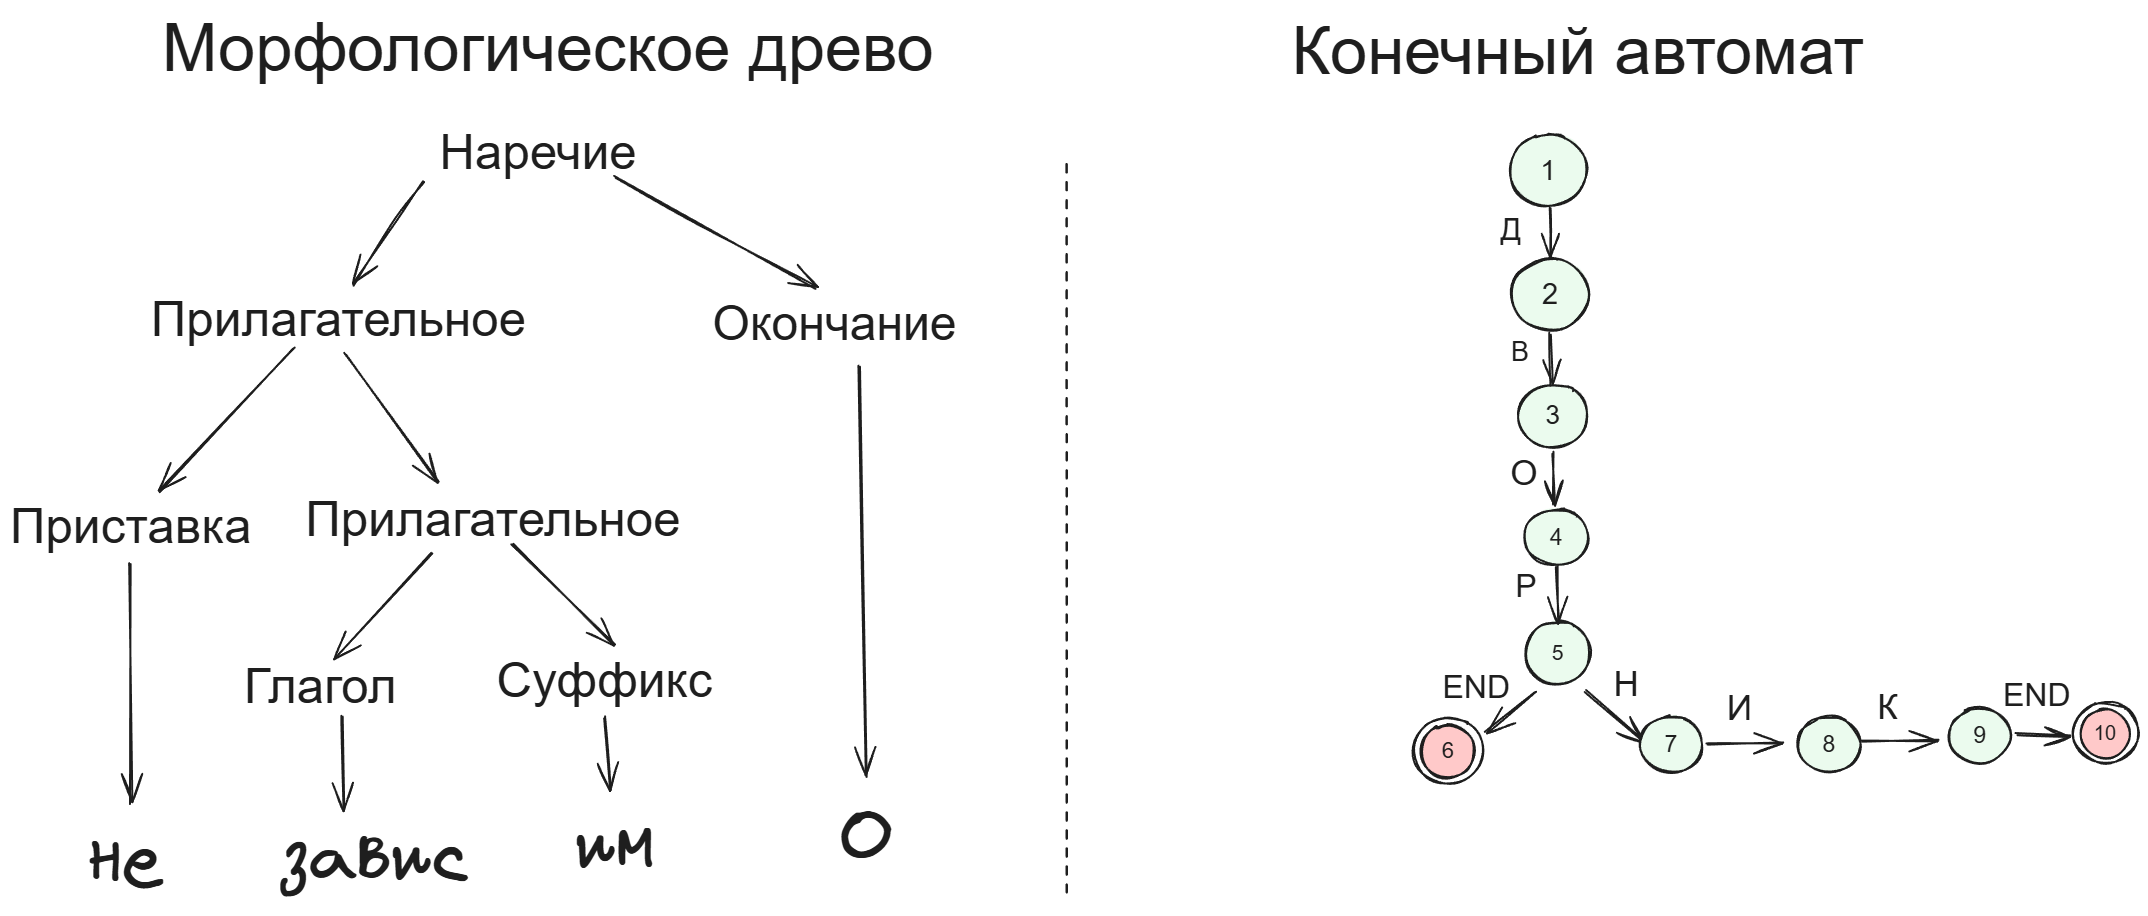
\includegraphics[width=0.5\textwidth]{assets/ml/nlp/morph_tree.excalidraw.png}
    \caption{Морфологическое дерево задает совместную иерархическую структура слова в виде конечного автомата.}
    \label{morph}
\end{figure}

Для обработки языка используются конечные автоматы, позволяющие выделять из набора символов строки в соответствии с запросом. 
Распространенным примером являются регулярные выражения, широко использующие для выделения ключевых слов в информационном поиске.

Для обработки естественного языка методами формальных языков из слов выделяются стем и словоизменительные парадигмы, являющиеся 
образцами для склонения или спряжения. Такие структуры создаются специалистами лингвистами и позволяют путем склонения,
спряжения и добавления приставки получать необходимые формы слов.

\textit{Определение:} \textbf{Морфологическим анализом} называют процесс разложения 
слова $w$ на его морфемы, например, префикс $P$, корень $R$ и суффикс $S$, из словаря $S$

\textit{Определение:} \textbf{Морфологическим синтезом} называется функция $f$,
формирующая слова $w$ из леммы $l$ и морфологических характеристик $m$. 
Примерами морфологических характеристик являются число, род, падеж.

Автоматическая обработка предложений выполняется путем выделения синтаксических связей.

\textit{Определение:} \textbf{Синтаксическое дерево} описывается как упорядоченное дерево $T$ с вершинами $N$, соответствующими
синтаксическими категориями (например, S, NP, VP), либо терминальному символу.

Получаемое дерево в качестве листьев представляет слова в предложении, а коренной узел $r$, заключает структуру предложения. 
Тогда дерево разбора $T$ для строки $w = w_1 w_2 \ldots w_n$ запишется как четверка $T = (N, E, r, L)$, где: 
\begin{itemize}
    \item $N$ --- конечное множество узлов;
    \item $E \subseteq N \times N$ --- множество ребер, каждое из которых соединяет пару узлов (родитель — потомок);
    \item  $r \in N$ --- корень дерева;
    \item $L = \{ w_1, w_2, \ldots, w_n \} \subseteq N$ --- множество листьев, соответствующих словам в предложении.
\end{itemize}